%!TeX root = 5-diffusion.tex
\documentclass[main]{subfiles}

\begin{document}

\chapter{Xenon and krypton transport properties}
\vspace*{-1\baselineskip}

\section{Current state of the art}

Experiment? \todo{reprendre la review daglar}

\subsection{Molecular dynamics}

\begin{figure}[ht]
    \centering
        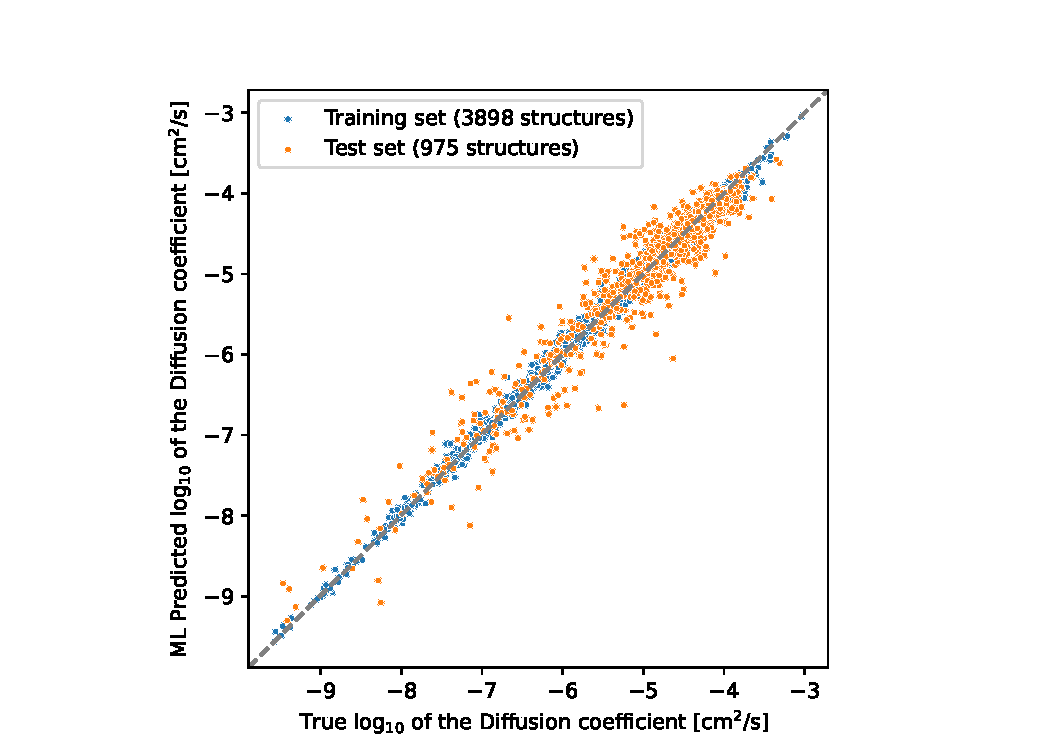
\includegraphics[width=6cm]{figures/5-diffusion/diffusion_prediction.pdf}
        \caption{}
        \label{fgr:}
\end{figure}

\begin{figure}[ht]
    \centering
        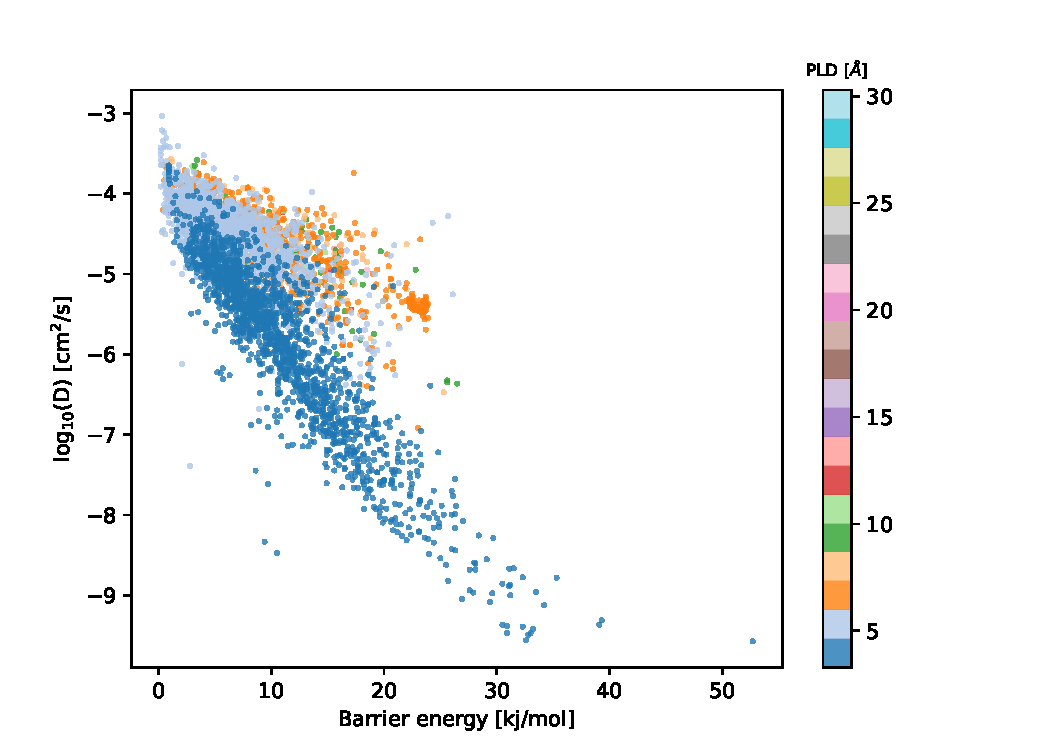
\includegraphics[width=0.48\textwidth]{figures/5-diffusion/difflog_barrier_Df_uff.pdf}
        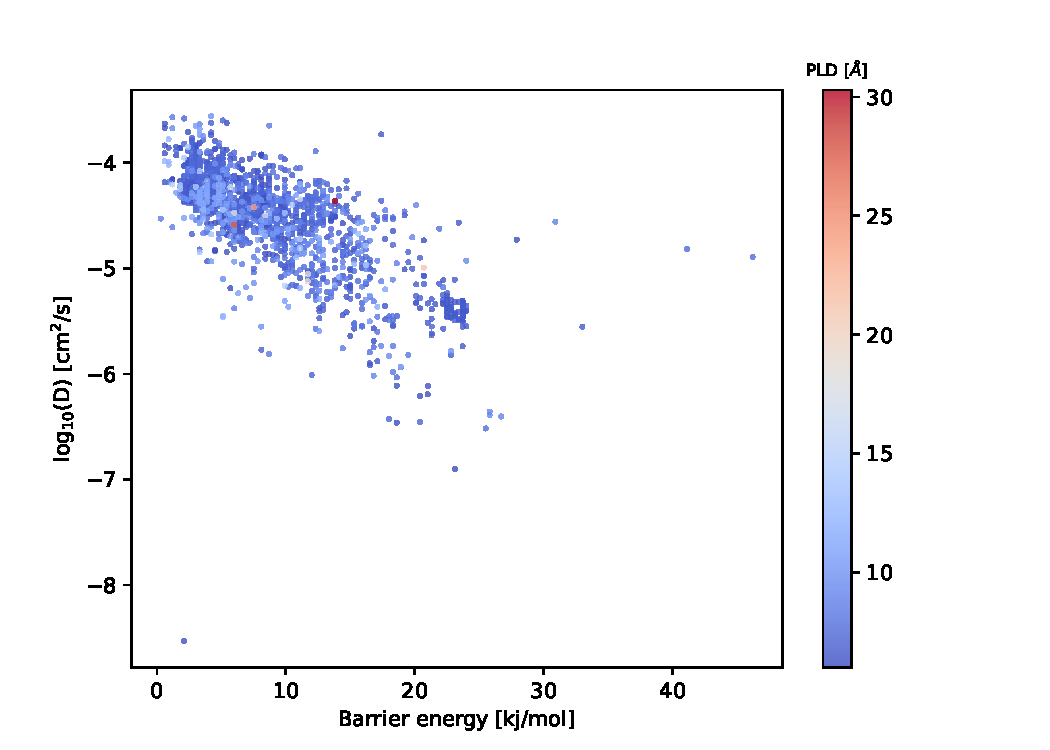
\includegraphics[width=0.48\textwidth]{figures/5-diffusion/difflog_barrier_Df_uff_2.pdf}
        \caption{}
        \label{fgr:}
\end{figure}

\begin{figure}[ht]
    \centering
        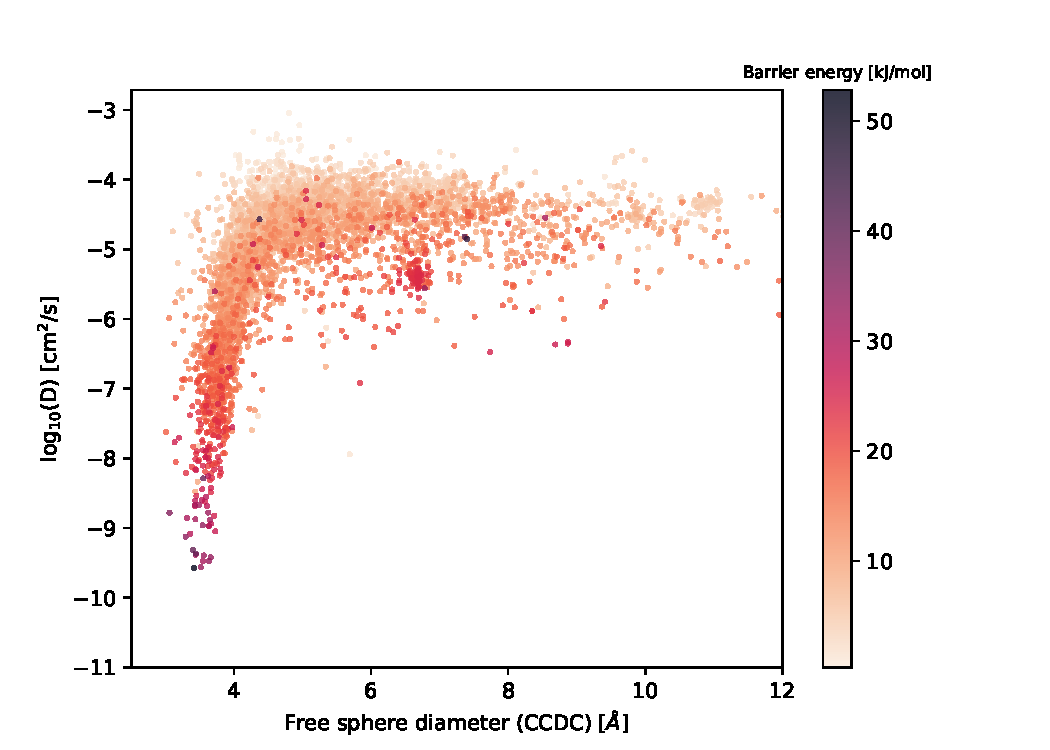
\includegraphics[width=0.48\textwidth]{figures/5-diffusion/difflog_Df-ccdc_barrier.pdf}
        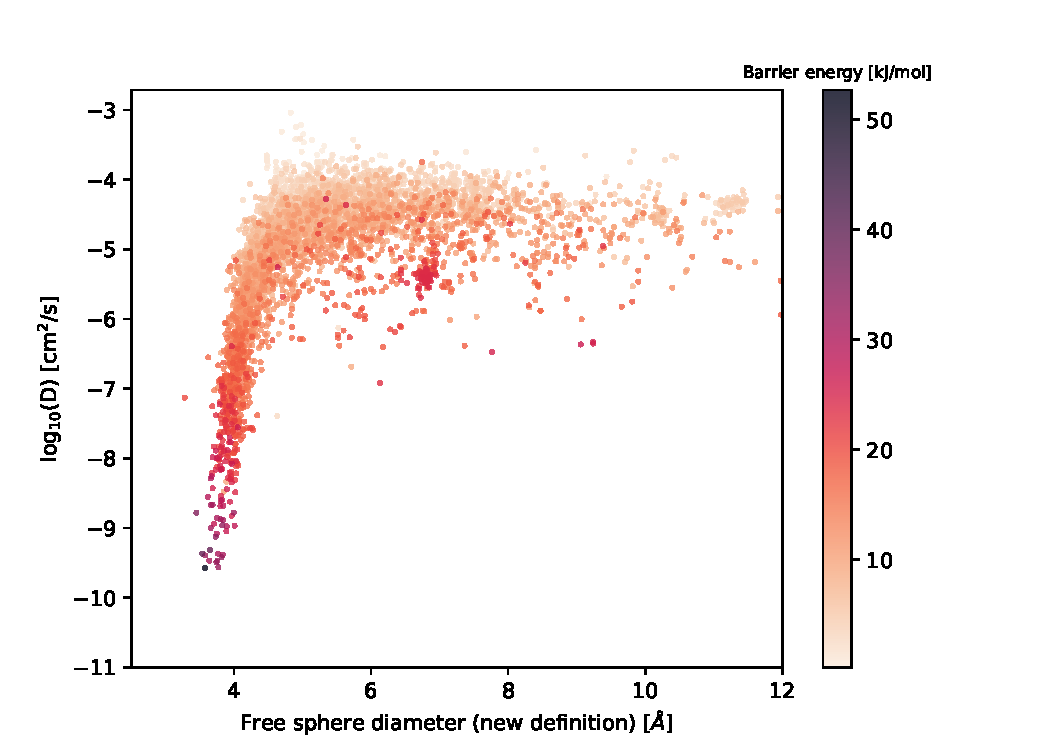
\includegraphics[width=0.48\textwidth]{figures/5-diffusion/difflog_Df-uff298K_barrier.pdf}
        \caption{}
        \label{fgr:}
\end{figure}

\subsection{Fast kinetic Monte Carlo}
tutrast
ctutrast\cite{Mace_2019}
ML descriptors
next steps

\section{ML modeling}

Results

\section{Molecular dynamics calculation results}

\subsection{Why is it relevant?}

\subsection{Correlations}

\section{Fast diffusion calculation algorithm}

\subsection{Implementation in C++}

\subsection{Preliminary results}

\subsection{Visualization tool}

\subsection{ML model training}

\OnlyInSubfile{\printglobalbibliography}

\end{document}
